\documentclass[12pt]{article}

\usepackage{sbc-template}

\usepackage{graphicx,url,multirow,textcomp}
\usepackage[caption=false]{subfig}

%\usepackage[brazil]{babel}   
\usepackage[latin1]{inputenc}  


%Comandos
\newcommand{\fig}[4][ht]{
  \begin{figure}[#1] {\centering\scalebox{#2}{\includegraphics{fig/#3}}\par}
    \caption{#4\label{fig:#3}}
  \end{figure}
}
     
\sloppy

\title{Receiving an amplified data from a biosensor via a wireless network}

\author{Andr� Ruza Paulon\inst{1} and Dr. Ant�nio Augusto Fr�hlich \inst{1}}


\address{Software/Hardware Integration Lab -- Federal University of Santa Catarina \\
  Florian�polis -- SC -- Brazil\\
  \email{andrerp@lisha.ufsc.br}}

\begin{document} 

\maketitle

\begin{abstract}
Biosensors are analytical devices for the detection of an analyte wich combines a biological component with a physicochemical detector component. They have been greatly developed in recent years for environmental monitoring. However, several technological deficits, such as to amplify a low voltage signals and mobility, hamper the growth of biotechnology sector. This paper proposal a tool to amplify a low voltage signals generated by a biosensor and  capture it over a wireless network that will contain a system capable of capturing, filtering and interpreting the transmitted data. The received signals from a hydroquinone sensor are compared to a potentiostat-galvanostat PGSTAT12 measurements to show the good accuracy that our system, significant cheaper and smaller, effectively achieved in order to contribute to the development of new technologies.
\end{abstract}
     
\section{Introduction} \label{sec:firstpage}

Biosensors can have a variety of biomedical, industry, and military applications. In spite this applications with tecnology do not be so abundant at market, it have tremendous potential for commercialization in other fields of application as well, this is due biosensors represent a promising tool to supplement existing techniques, due to its unique characteristics, such as selectivity, relatively low cost of construction and storage, potential for miniaturization, ease of automation equipment and construction of simple and portable for a quick monitoring\cite{ROSATTO2001} . However, commercial adoption has been slow because of several technological 	difficulties. For example, due to the presence of biomolecules along with semiconductor materials, biosensor contamination is a major issue. \cite{Mohanty2006}.

Besides research in the area discovered and improved technologies like glucose meters, pulse rate and temperature, a new demand for sensors is emerging trending to increase problems like the topologies that are used and that influence the distribution of sensors, the limited capacity of the batteries, the materials used and the consequences they generate in the environment which they are exposed, the development of software capable of operating with low memory, filter a low frequency signal\cite{Lili:2009}, resulting in problems of how to handle the data and how to obtain them.

Technologies used in the management of biosensors tend to be big, expensive and delicate due to parameters imposed by them cited previously, difficulting  mobility in the applications.The implementation of Wireless Sensor Network (WSN) with biotechnology can greatly contribute to the advancement of new applications and technologies.

Wireless Sensor Networks have proliferated rapidly in the last few years. These networks enable the monitoring of a variety of potentially harsh environments and can be used for continuous sensing, event detection, event ID, location sensing, and local control of actuators. The concept of micro-sensing and wireless connection of these nodes promise many new application areas. \cite{Akyildiz:2002} categorize the applications into military, environment, health, home and other commercial areas. It is possible to expand this classification with more categories such as space exploration, chemical processing and disaster relief. 

Currently there is an increasing interest on applications composed by autonomous and cooperative devices that requires reliable monitoring, precise, foolproof and  preferably in real time. These applications are formed by a variable number of nodes, which interact through a wireless communication network to exchange control, status, and possibly stream messages. Most of these messages have real-time and quality of service (QoS) requirements, such as time limits to deliver messages, temporal validity of data, and synchronization requirements (delay variation limits) \cite{Sobral:2008}. 

In this paper we present a proposal for amplifing a low voltage of electrical signals generated by a hydroquinone biosensor and  transmit it over wireless network that will contain a system developed to filter and interpret the transmitted data. At the end will be compared the received signals to a data performed on a potentiostat-galvanostat PGSTAT12 to show what  has,  effectively, contributed to the development of new technologies in a simple and inexpensive.

This paper is organized as follows. Related work in section 2. In section 3, we will present a description of the implemented architecture. A brief overview about the biosensor used in Sections 4. A Presentation of the filter described in Sections 5. The results obtained are presented in section 6. And finally, we explain our conclusion in Section 7.

\section{Related Work}
In this section we will present the projects which have some relevance for this experiment and how they helped us reach our goal.

In the Salerno University, \cite{Albanese2010} an innovative measurement system for automatic FIA(Flow Injection Analysis) is proposed. It has a local measurement units and a central control unit. The main innovations are concentrated in the digital signal processing: peak amplitude measurement is fully automatized because the proposed units are able to detect the correct peak. The biosensor characteristics can be memorized in order to provide the analyte concentration as result. Furthermore, the LMU's (Local Measurement Unit) can be interfaced via RS485 port to a controller in order to be used in a multisensor measurement system for FIA process automatic management. A novel unit playing the role of controller (Manager Unit) has been designed to control several LMU's and a set of actuators, e.g. pumps and valves. Nevertheless, the communication between LMU and MU can be realized through a serial link.

An experience supported by Chinese Academy of Sciences \cite{Wang:2010} describes the development of a wireless biomedical sensor interface system-on-chip (SOC) that aims to combine many of the functions of the BSN microsystems onto a single substrate. The design is specified for a biosensor system with up to eight pH and temperature data channels communicating via an encoded wireless interface to a remote base station. The system comprises analog sensor interface circuit, data-conversion circuits, a microcontroller, a data encoder, and a frequency-shift keying (FSK) RF transmitter. However it takes experiments \cite{Chirwa:2003}, \cite{Wang:2007} , which report bioeffects, into account. Bioeffects, such as signal absorption by the organism can impair efficiency of a small antenna in enviromental measurements.

 In \cite{Steinberga2009}have been developed a short-range wireless RF tag capable of measuring pH and sending that data to a nearby reader. The tag contains a pH sensitive optrode that exploits the differential absorbance of light in a thin-film of bromocresol green indicator dye at two wavelengths. The measurement wavelengths correspond to the isosbestic point and the pH sensitive peak of the optical absorbance curve. The sensor is responsive over the range from 5.2 \textendash 8.3 pH units. Because the wireless system is based on the ISO standard RFID platform, it could in the future be suitable for use as a chemical and biological detector in different industries where this standard has been adopted. By adapting and modifying the specific indicator chemistry and optoelectronic detector measurement strategy, the platform could be deployed for different chemical and biological analytes, in addition to just pH. Conversely, The RFID reader energises and communicates with passive tags wich  do not contain a battery or power supply, but operate by scavenging energy from the electromagnetic  field generated by the antenna connected to the reader. Beside that, these passive devices do not generate machinereadable digital data, they do not easily scale from one to ''many'' devices, and cannot form or join wireless networks. Because they lack a core microprocessor, the devices cannot be programmed to conform to any of the established wireless protocols, which is a serious limitation to their widespread adoption.

\section{Local measurement unit}

This experiment was composed by three main parts: Sensible element, Conditioning circuit and Processing unit. Its schematic is showed in Figure 1. The Sensible element (the biosensor) is constituted by a sensitive biological element (immobilized enzyme) within an electrochemical cell; it converts the
analyte under test in a current. The Conditioning circuit converts the current signal in a voltage signal which is measurable by the processing unit. The acquired voltage is processed to evaluate the analyte concentration\cite{Liguori:2009}. In the Processing Unit we use a EPOSMote that transmit the data via radio to a supervisor PC interacts with measurement unit for displaying measured results and helping the user manage the calibration procedure. 

\vspace{3.5 cm}
\begin{figure}[!htbp]
     \flushleft 
%     \centering
     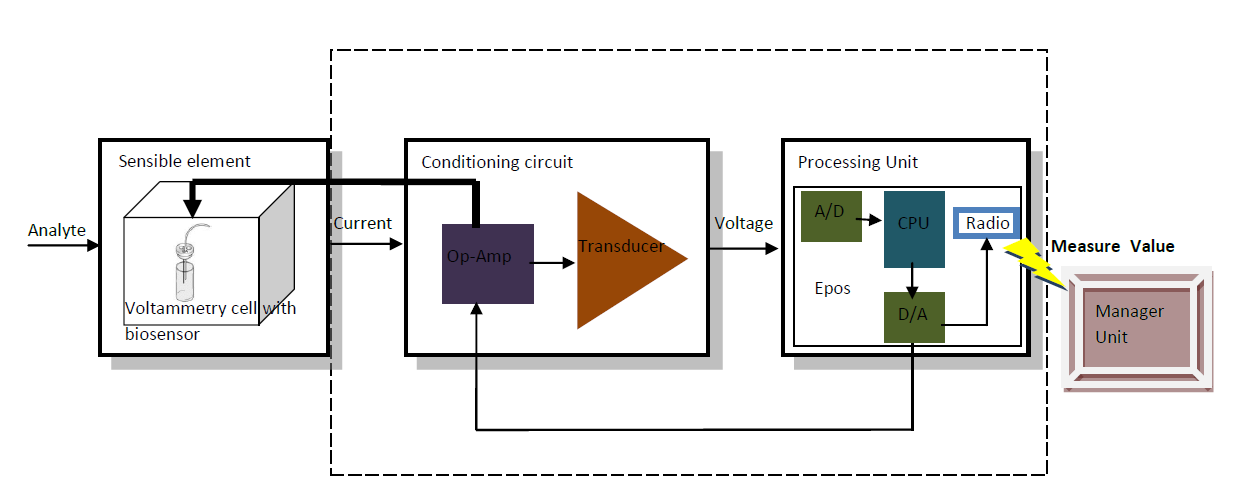
\includegraphics[scale=0.37,bb=1 1 400 94]{imagens/LMU.png}
     \caption{Block diagram of the Local Measurement Unit(LMU)}
     \label{Fig1}
\end{figure} 


\subsection{Sensible element}
The sensible element consists by three electrodes working in a voltammetry cell  to have a controlled potential. The working electrode (WE) which works as the cathode, and the reference electrode (RE) which is the anode. Thus, electrons go out from the cathode into the solution, being attracted by the anode. To make the result obtained repeatable, it is essential for the difference of potential between both electrodes to remain constant. However, as soon as current passes through the reference electrode (usually a silver wire) it gets polarised, which means that its potential will vary with this current. Hence, to maintain a stable potential no current is allowed to pass by the RE electrode.

To avoid this drop of voltage a third electrode is added to the electrochemical cell: the auxiliary electrode (AE), in this case is used a carbon tube with a contatct area bigger than the work electrode, which acts as an anode as you can see in Fig. 2. A current is forced between WE and AE, high enough and in proper polarity to keep the working electrode potential at a constant value with respect to the RE electrode\cite{Blanco:2006}.

\vspace{2.5 cm}
\begin{figure}[!htbp]
     \centering
     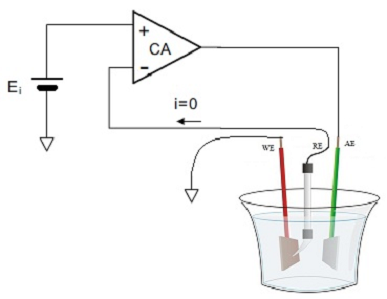
\includegraphics[scale=0.6,bb=0 0 200 94]{imagens/Potenciostato2.png}
     \caption{Voltammetry cell with three electrodes}
     \label{Fig2}
\end{figure}

\subsection{Conditioning circuit} 
Figure 3 shows the conditioning circuit projected as a potentiostat. This circuit consists of a I-V converter, that transforms the output voltage to be proportional to the current generated in the electrochemical cell, and so it is directly proportional to the concentration of analyte in the solution. 

\vspace{3 cm}
\begin{figure}[!htbp]
     \centering
     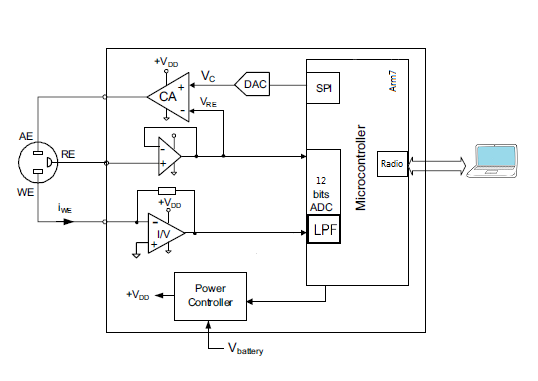
\includegraphics[scale=0.6,bb=0 0 400 94]{imagens/AmpopCircuit.png}
     \caption{Voltammetry cell with three electrodes}
     \label{Fig3}
\end{figure}


In order to measure these low levels of current, an operational amplifier with a very low offset current, low noise and great input impedance will be necessary. In the feedback loop it is useful to put a small capacitor for the phase compensation and eliminating high-frequency noises.

%Was used two different op-Amp in order to compare wich of them will better provide our purpose.

%At first the signal was amplified by a op-Amp TL082, represented in Figure 4, sensitive to a input bias current up to 50$-$400 pA, a large signal voltage gain 25$-$100 V/mV,  15 mV ofInternally trimmed offset voltage, low input noise voltage 16nV/vHz, low input noise current 0.01 pA/vHz High input impedance $10^{12} \Omega$ \cite{website:TL082}, so depending the current generated by sensor we may need  an amplifier with a higher capacity of amplification, but with the same level of sensitivity.

%\vspace{1.5 cm}
%\begin{figure}[!htbp]
%     \centering
%     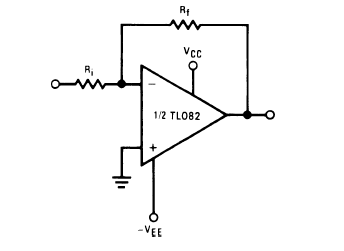
\includegraphics[scale=0.5,bb=0 0 200 94]{imagens/Ampop.png}
%     \caption{Typical Connection}
%     \label{Fig4}
%\end{figure} 

In our test we use a INA116, represented in Figure 4, with a lower input bias currents of 3fA at 25\textdegree C, and only 25fA at 85\textdegree C. Its 3$-$op amp topology allows gains to be set from 1 to 1000 by connecting a single external resistor.The INA116 is available in 16$-$pin plastic DIP and SOL $-$16 surface-mount packages, specified for the $-$40\textdegree C to +85\textdegree C temperature range\cite{website:INA116} which provides us with an increase in the range of biosensors that can be used in this circuit.

\vspace{3.5 cm}
\begin{figure}[!htbp]
     \centering
     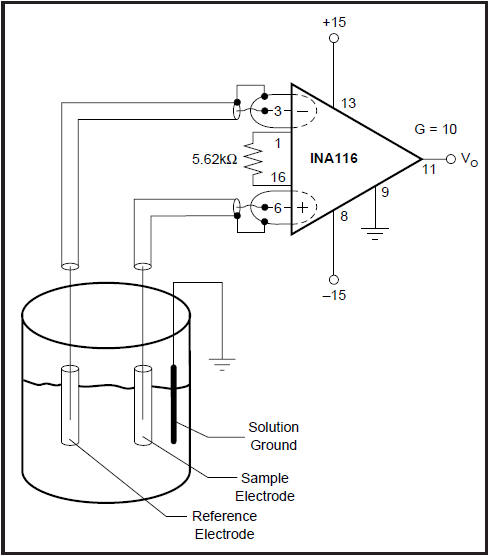
\includegraphics[scale=0.3,bb=0 0 400 94]{imagens/MeasurementSystem.png}
     \caption{Typical Connection}
     \label{Fig4}
\end{figure} 

\subsection{Processing unit}
The signal acquisition, conversion and processing is carried out by a ARM7TDMI microcontroller (by ARM) that is featured with analog to digital (ADC) converter where a low pass filter is is employed in order to filter the low frequency noises of the collected information. The gain generated by conditioning circuit that is controlled by a digital microcontroller output that will be converted by a DAC and returned to CA.    

The chosen PiP (Platform-in-Package) was the Freescale MC13224V, it's based in an 32-bit ARM7 core and your major features include an integrated balun for an easy antenna matching circuit, a built-in radio, 128Kbyte flash memory, 80Kbyte rom memory, 96Kbyte RAM memory and an integrated PA which provides programmable output power from -30dBm to +4dBm, all this in a 9.5x9.5$mm^2$ footprint. Moreover it owns low power consumption supply voltage 2.0 - 3.6 V,-96dBm for 1\% RX sensitivity, high-density memory bandwidth 2.4 GHz ISM, with many different interfaces: 2 UARTs,2 individual ADCs with 8 input channels and a 12-bit resolution, SPI, SSI, KBI.\cite{website:EposMote}

The communication between LMU and manager unit (MU) is realized through wireless link via WSN. EPOSmotes  can perform data transmission to an average distance of 20-100 meters depending on the terrain and obstacles in the middle.

The potentiostat working voltage value, generated by the DAC output, depends on the single biosensor in our cause the best operating voltage for a hydroquinone biosensor is 50mV as the measure presented in Table 1.	

\subsection{Manager unit}
A system, developed in python, installed in the data receiver is able to interpret the received data and plot graphs, facilitating remote monitoring without the need of wires. This would allow, for example, to effectively utilize these technologies in order to improve the processes involving chemical measurements such as wine production, use of pesticides in agriculture, food production, among others.
%Trocar pelo labview

\section{Used Biosensor}
The implemententation of LMU was started by means of amperometric biosensors for the determination of hydroquinone using a carbon paste electrode owing to important advantages to all other solid electrodes. The speed and simplicity of the preparation process, and the possibility of renewing the electrode surface with each new measure. This is  important in the analysis of compounds where the reaction products are adsorbed on the electrode surface. Another important property is the low residual current, which is lower than that for pyrolytic graphite electrodes and carbon vitreous. Howerver arise some difficulties to determination of substances with a carbon paste electrode is its high detection limit, which complicates the analysis of trace substances\cite{Marcolino:2007}.

\subsection{Electrochemical measurements}
The voltammetric measurements were performed on a potentiostat-galvanostat PGSTAT12 the Autolab (Eco Chemie, Sweden) using a software GPES version 4.9.006, Eco Chemie, see Figure 3. A glass cell with PVC cover was used without dividing compartment containing 10 mL of acetate buffer 0.1 mol L-1 (pH 5.0) with aliquots of standard solution of hydroquinone. The three electrodes used were constructed using the biosensor as working electrode, a platinum plate (0.5 cm2) electrode used as auxiliary electrode and Ag / AgCl (3.0 mol L-1 KCl) as reference electrode.

In Table 1, the electrochemical measurements realized is reported, indicating the potential and current according to the concentration of the solution for the volume of hydroquinone injected into the cell.
 
\begin{table}[ht!]
\begin{center}
\begin{tabular}{|p{2cm}||p{3cm}||p{2cm}||p{2cm}||p{2cm}||p{2cm}|}
\hline
\textbf{Volume of the aliquot} & \textbf{Concentration of hydroquinone (mol / L)} &\multicolumn{2}{|c|}{Square wave voltammetry} &\multicolumn{2}{|c|}{Cyclic voltammetry} \\
\hline
 &  &  Current & Potencial & Current & Potencial\\
\hline
50  uL &	3,01x10-5 & 2,733x10-7 & +0,289 & 1,43x10-7 & +0,357\\
\hline
100 uL & 5,95x10-4 & 5,079x10-7 & +0,304 & 3,06x10-7 & +0,362\\
\hline
150 uL & 8,88x10-4 & 7,595x10-7 & +0,304 & 4,59x10-7 & +0,352\\
\hline
200 uL & 1,18x10-3 & 9,97xx10-7 & +0,313 & 6,08x10-7 & +0,348\\

\hline
\end{tabular}
\end{center}
\caption{Electrochemical measurements realized on a potentiostat-galvanostat PGSTAT12}
\label{Tab1}
\end{table}

With the measures outlined above a graph of current through the power can be generated to facilitate the understanding of the sample as shown in Figure 6, and a square wave voltammetry as shown in figure 5.


\vspace{3 cm}
\begin{figure}
   \centering
	\subfloat[Cyclic voltammetry]{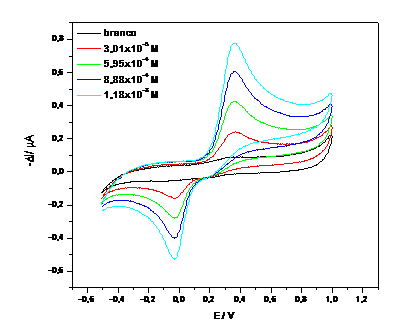
\includegraphics[scale=0.6,width=7cm,bb=0 0 400 94]  {imagens/VoltametriaCiclica.png}}\label{a}

	\vspace{3 cm}

	\subfloat[Square wave voltammetry] {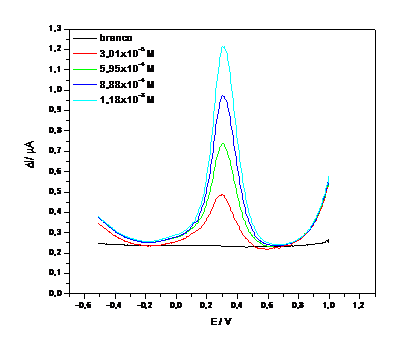
\includegraphics[scale=0.6,width=7 cm,bb=0 0 400 94]{imagens/VOQ.png}} \label{b}
	\caption{(a) Cyclic voltammetry with velocity of 500 mV/s and Potencial between -1,0 to +1,0 V.(b) Square wave voltammetry with frequency of 100 Hz, amplitude = 50 mV and a Increment = 5 mV/s and Potencial between -1,0 to +1,0 V.}

\label{fig7}
\end{figure}

%\vspace{3 cm}
%\begin{figure}[!htbp]
%     \centering
%     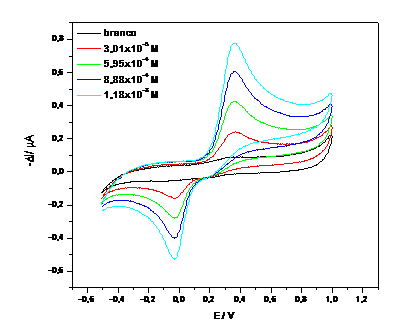
\includegraphics[scale=0.6,bb=0 0 400 94]{imagens/VoltametriaCiclica.png}
%     \caption{Cyclic voltammetry with velocity of 500 mV/s and Potencial %between -1,0 to +1,0 V.}
%     \label{Fig5}
%\end{figure} 

%\vspace{3 cm}
%\begin{figure}[!htbp]
%     \centering
%     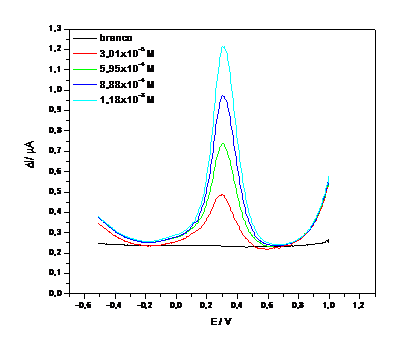
\includegraphics[scale=0.6,bb=0 0 400 94]{imagens/VOQ.png}
%     \caption{Square wave voltammetry with frequency of 100 Hz, amplitude = 50 %mV and a Increment = 5 mV/s and Potencial between -1,0 to +1,0 V.}
%     \label{Fig6}
%\end{figure} 

\section{Filtering}

Since the physiological or important information parameters are embedded in the waveform of the sensor signal, accurate and non-distortive sensor signal waveform extraction requires digital filter models which give a high magnitude attenuation for out-of-band frequencies and unwanted additive noise signal while preserving the linear phase characteristic of the filter to avoid distortion in the important sensor signal waveform\cite{Nkosi:2011}.
 
For our porpouse a low pass filter is employed in order to filter the low frequency noises since the sensor signal works in a high frequency. Overall, the implementation with the best properties seems to be the IIR\cite{Ban:2006}, wich better suit the MP ARM7TDMI.

\section{Experimental Results}

To prove the effectiveness of the experiment, whole system was
evaluated in the real case scenario using a hydroquinone biosensor that would be coupled to an amplifier wich raise the voltage obtained at a level that can be understood by  the ADC's of Eposmote and transmitted to the receiving node, from there a system developed in python makes sure that the information transmitted from the radio to the USB will be plotted on a graph, Figure 7.

In order to send the data with all necessary information, we had to implement a protocol that could send a Integer number indicating the voltage picked up at the time and use, after transfer the data via radio, to plotting of graphs in  receiver.

\vspace{3 cm}
\begin{figure}[!htbp]
     \centering
     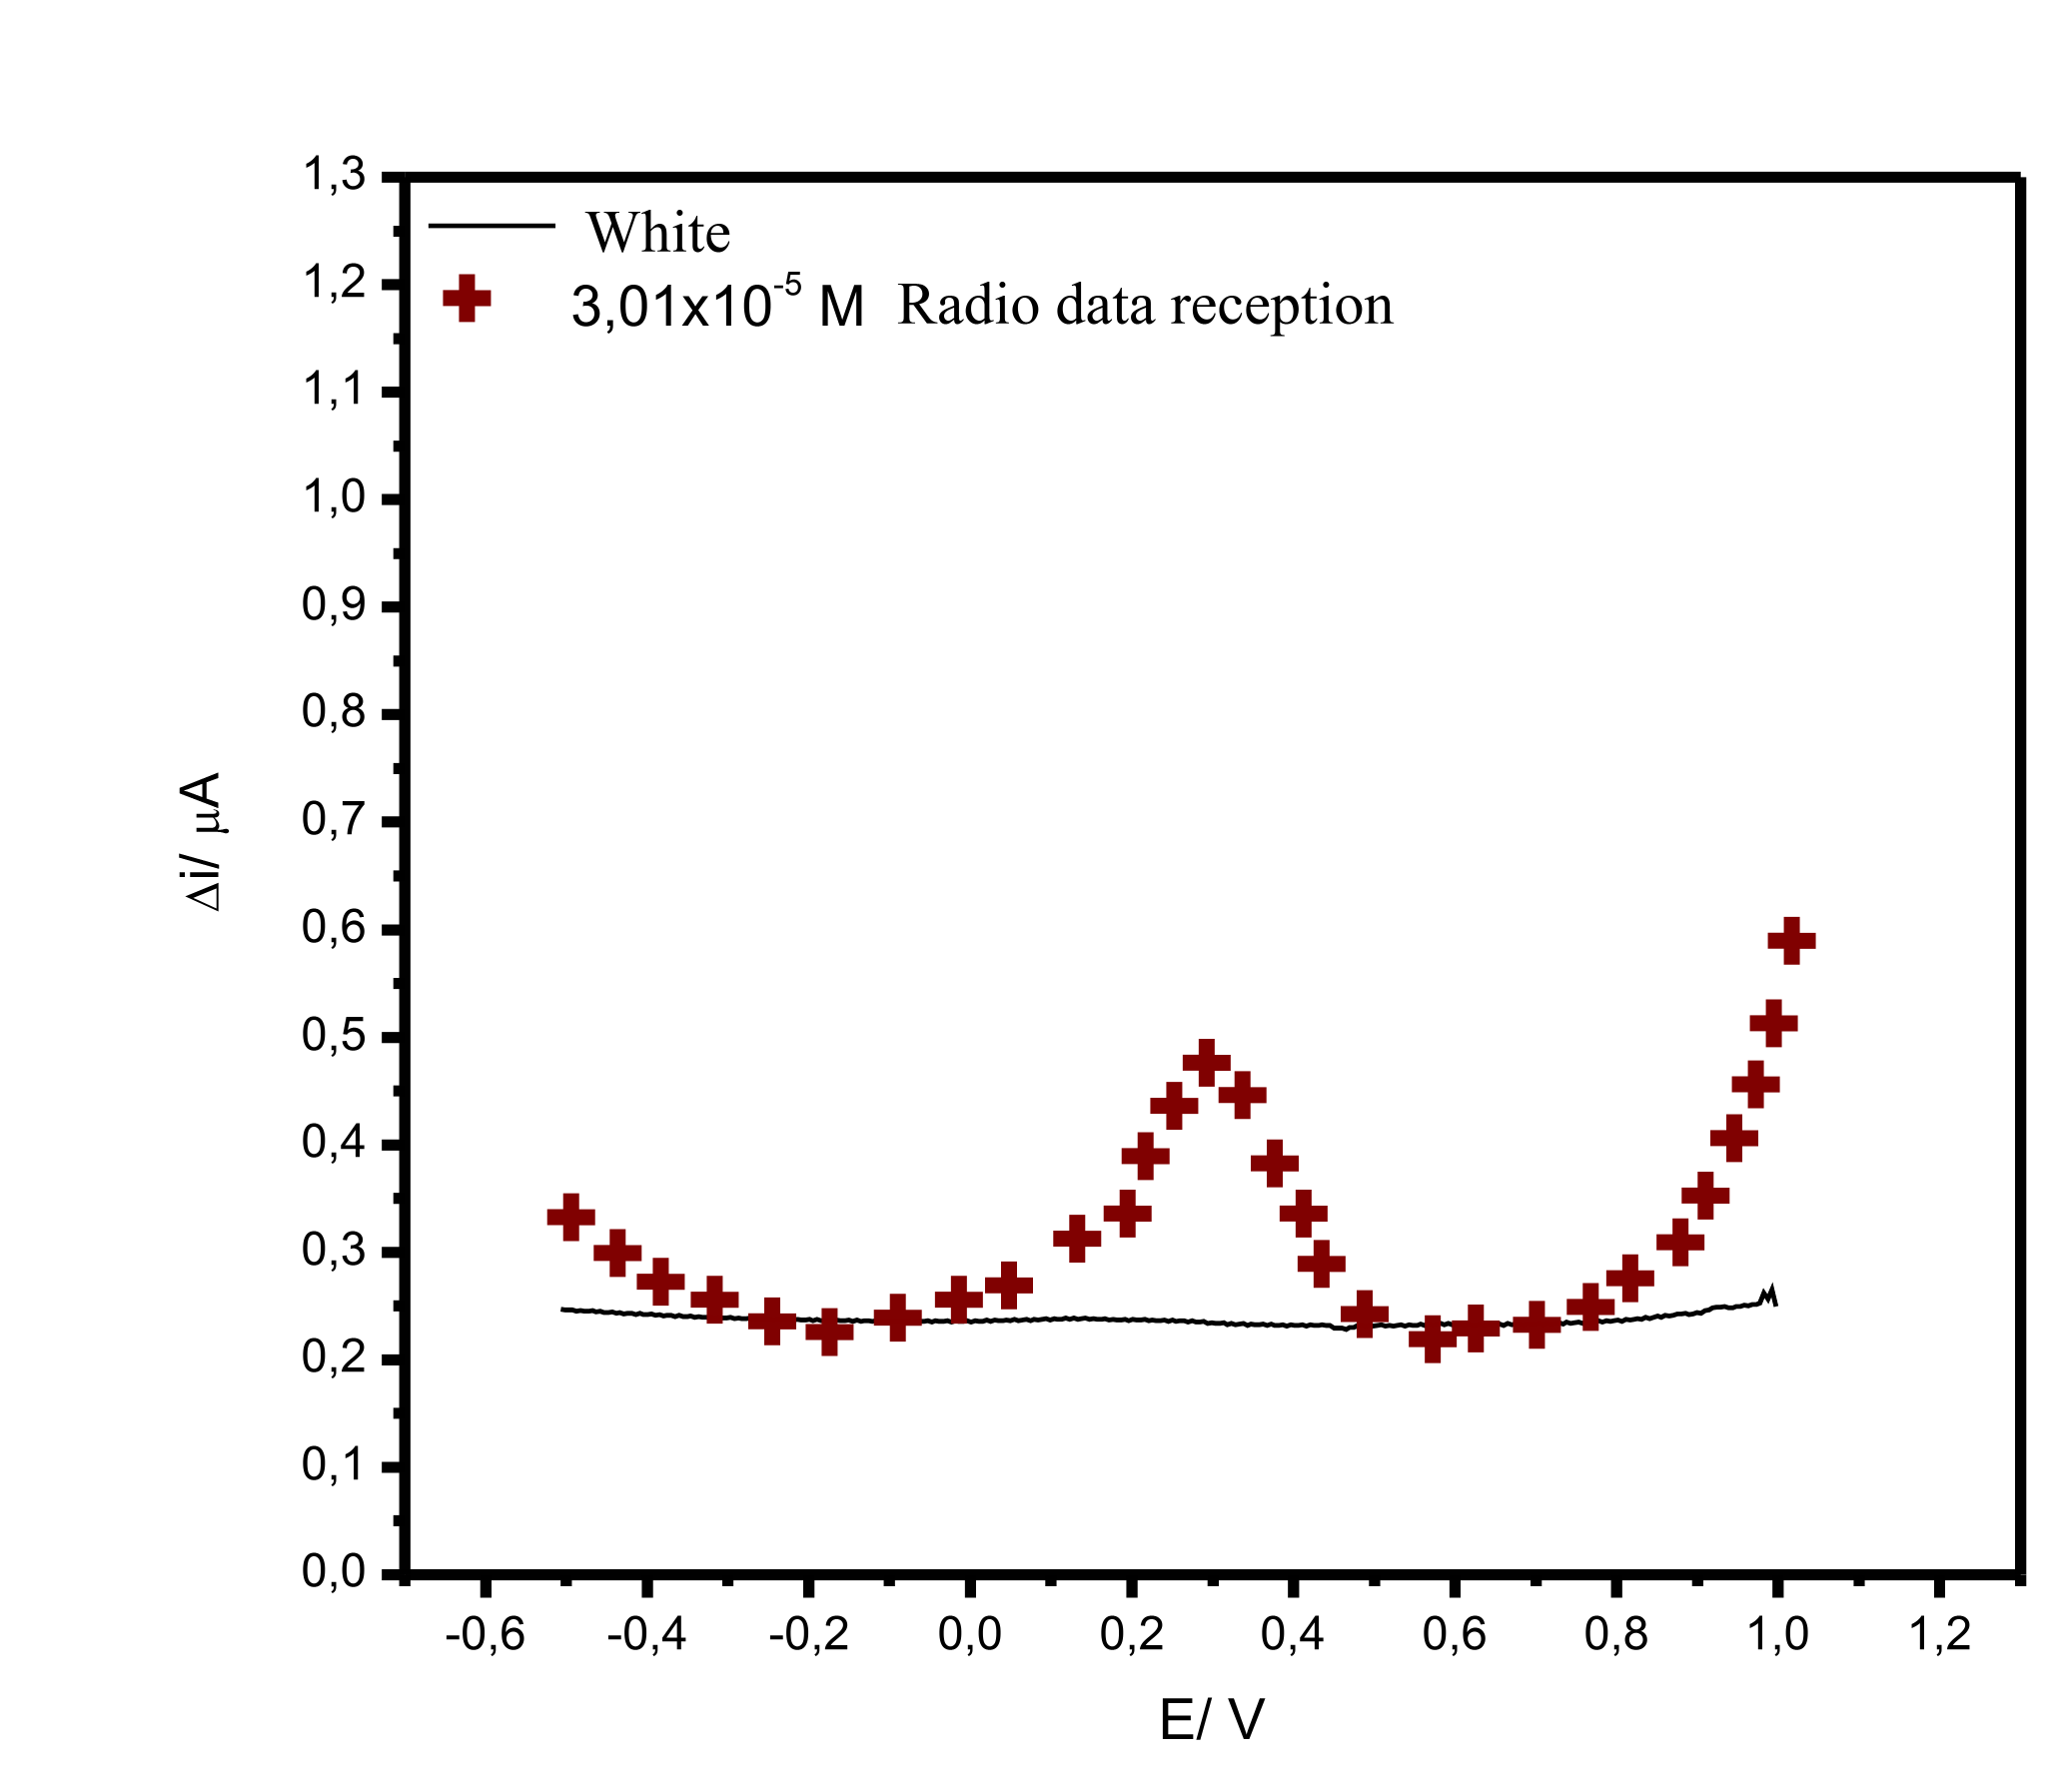
\includegraphics[scale=0.6,bb=0 0 400 94]{imagens/CompPotenciostatoVOQ.png}
     \caption{Graph obtained from the data received by radio}
     \label{Fig7}
\end{figure} 
 
In this graph we can see two discrete lines, the red line represents the regime flow, and the red crosses is the current flow data received by radio containing peaks that represent the chemical reactions that occur in a biossensor. 

Comparing the realized measurement with Figure 7, we note that the current flow are increasing at the same time as the measure from PGSTAT12 demonstrating that it is able to exhibit a constant performance. The LMU  implemented  can keep the same accuracy and even improving the reliability which can be obtained by any industrial systems as shown in Figura 9.

\vspace{3 cm}
\begin{figure}[!htbp]
     \centering
     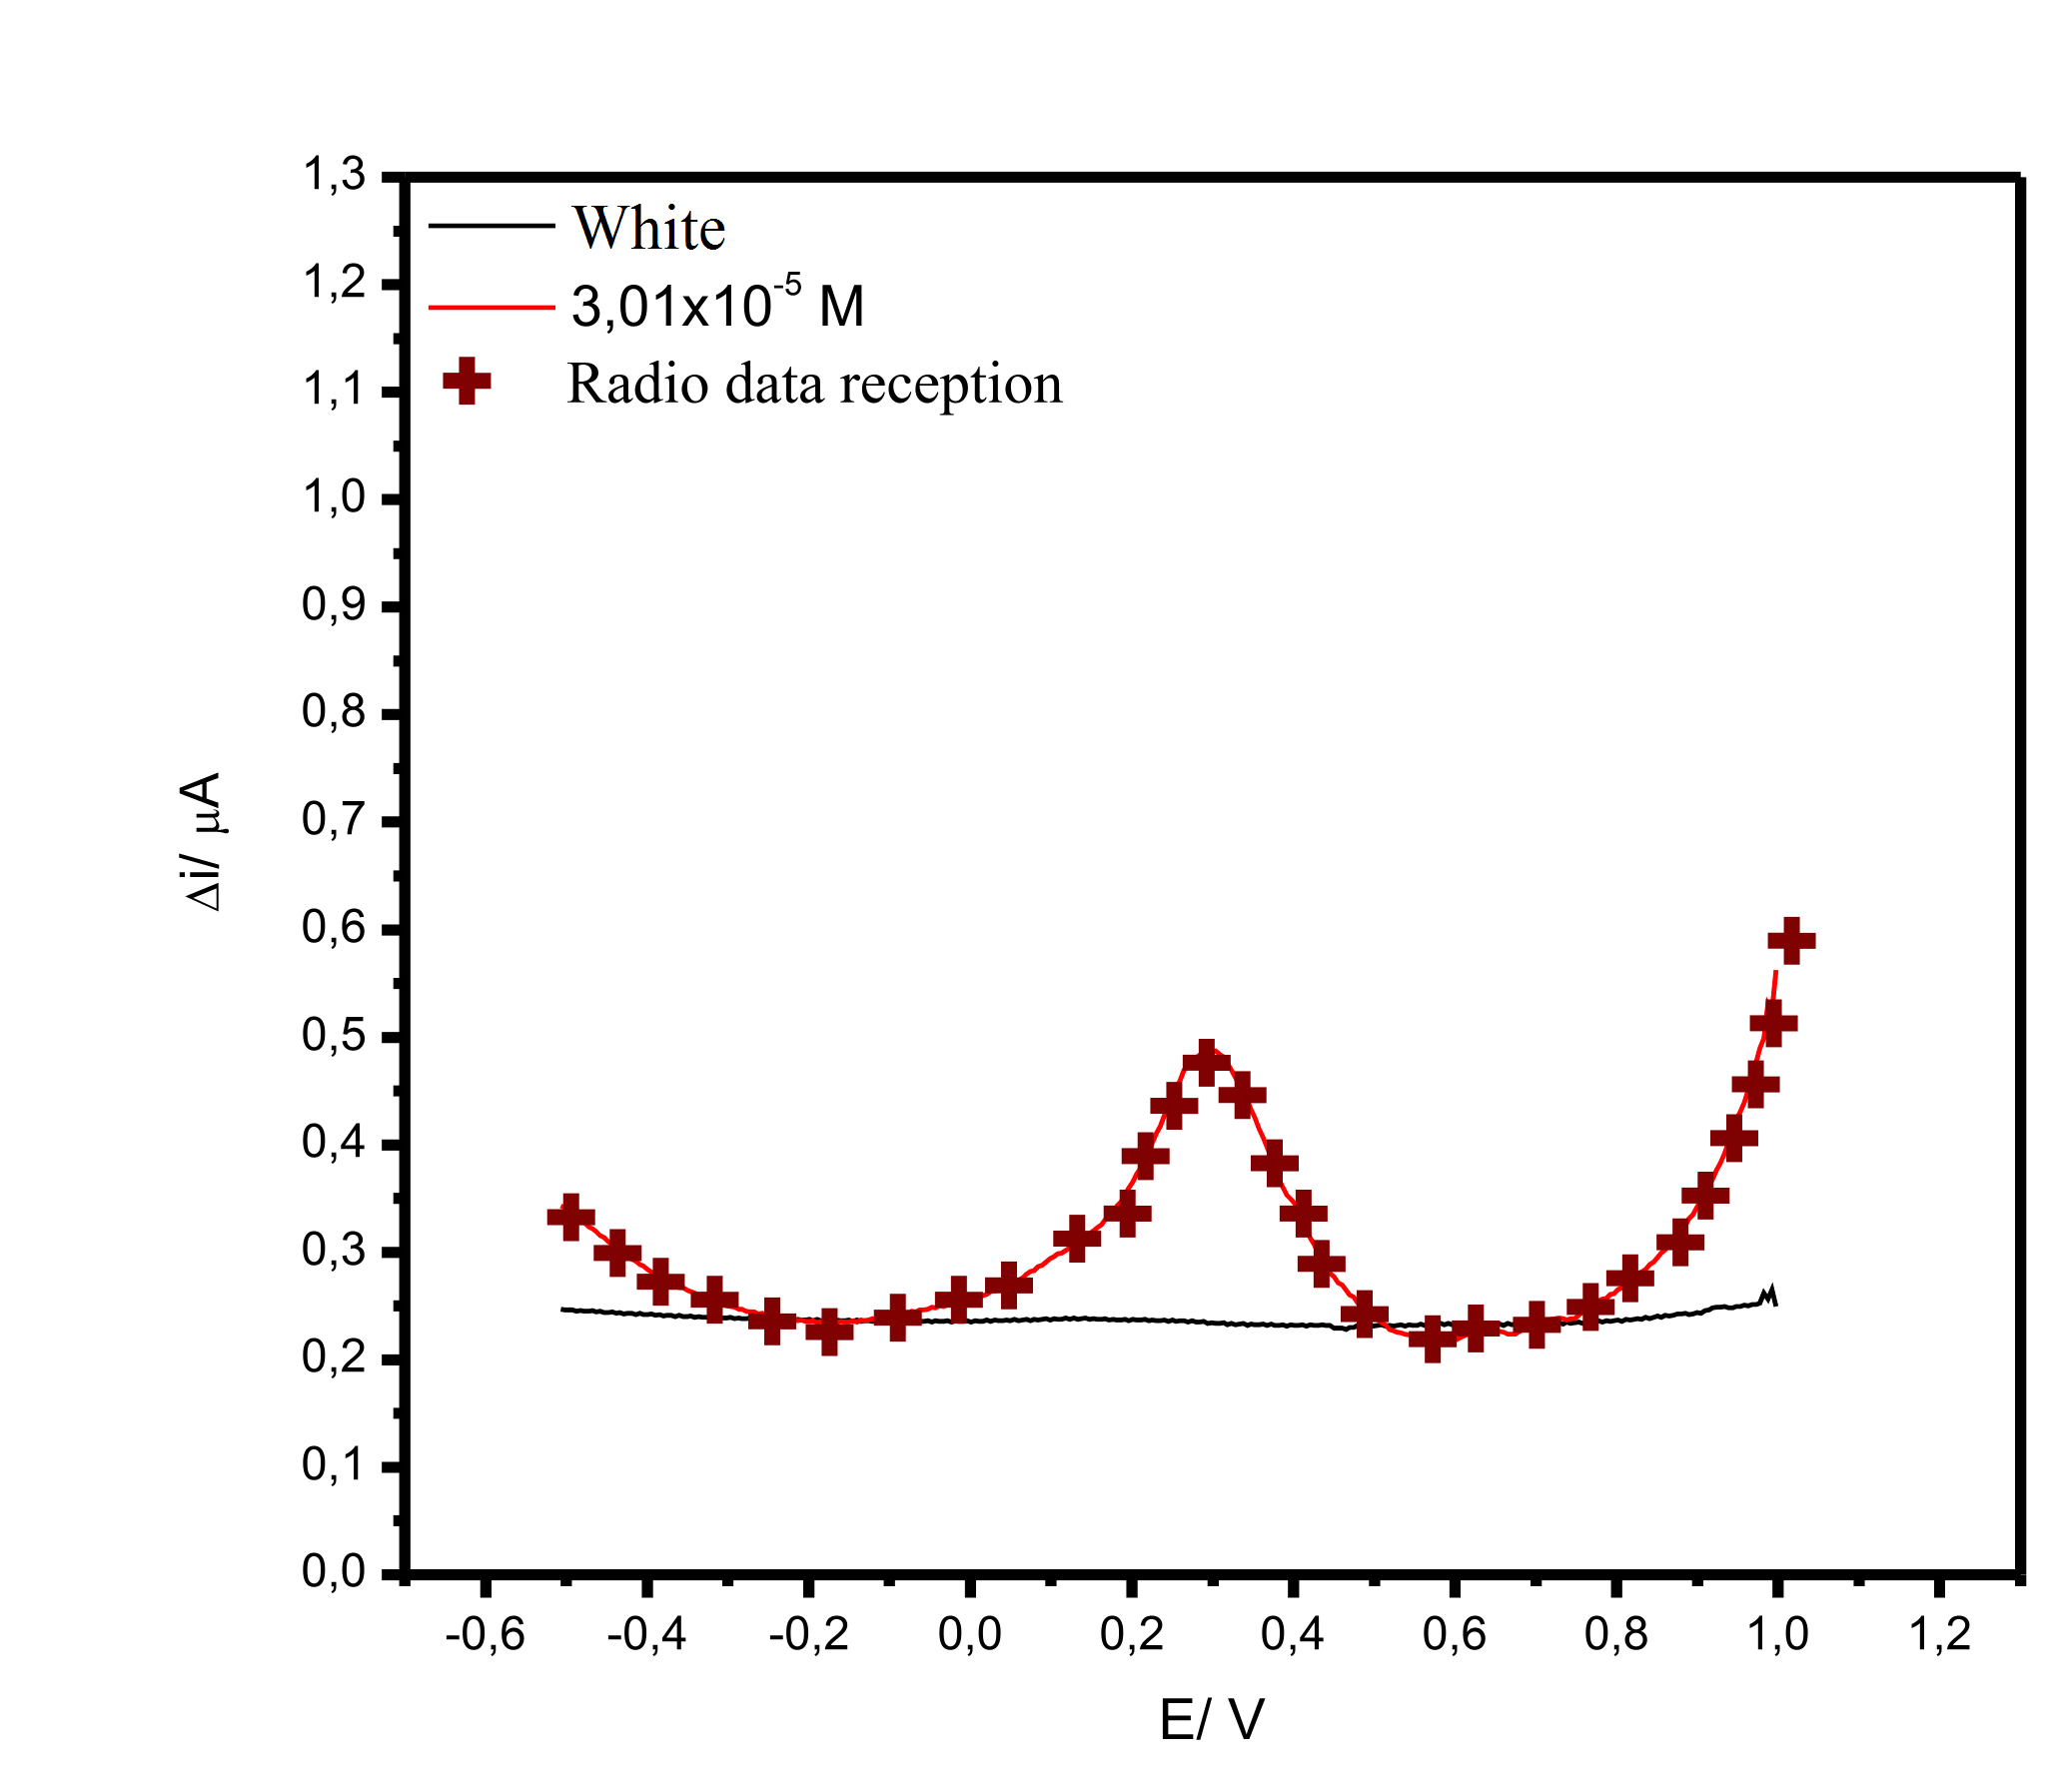
\includegraphics[scale=0.6,bb=1 1 400 94]{imagens/RadioReception.png}
     \caption{Comparation between PGSTAT12 and the developed system results}
     \label{Fig8}
\end{figure}

All summarizing, the data were properly sent and received with sufficient quality and accuracy that the experiment can help biosensors to be more and more largely used.

\section{CONCLUSION}

To achieve the goal, we present the design of a low-cost portable instrument for amperometric chemical sensors. It was tested by means of amperometric biosensors for the determination of hydroquinone. A methodology based on the presentation and development of a technology project that aims to detect a concentration of an analyte  by sending it via a wireless network for this information to be used in the receiver that will manipulate it according to need. In order to obtain a high precision solution, a low pass filter was implemented. Its noise level is low enough to measure dc currents with a resolution of 50 pA to 25fA.In addition, because the reduced size, low cost, battery-powered and WSN interface it is suited to be used directly in field applications..

It is a computer system that assists in obtaining measurements, improved productivity, ease storage of information that can result in a historical, research enabling better accuracy in determining the time between data collection.

In the future projects is desirable improve this sensibility and create a thorough protocol to send data without transport restrictions testing with different types of biosensors.

%\section{References}
\bibliographystyle{plain}
%\nocite{*}
\bibliography{Biosensor2}

\end{document}
